%!TEX root = ../proceedings.tex
% \subsection{Customer Expectations}
\textit{Clear expectations of all participants in trade benefit all, but introducing those expectations can be difficult for all parties.}

Perhaps the most common source of dissatisfaction with gig workers comes from a miscommunication or simply a mismatch in the expectations of the customer and the worker.
The effects of this mismatch appear to have been discussed when discussing Mechanical Turk, leading to norms where ``good" requesters know to provide examples of correct work and highlight common mistakes, explicating the intent of the micro work.
On other platforms, clear expectations are established ahead of time
(on ride-sharing markets, the expected driving path, estimated time, and estimated cost is displayed to customers).

People we spoke with at organization B, organization E, and organization C felt that formalizing the expectations of workers was the most appropriate solution to this problem.
By making it clear to customers what workers are expected to do
(for instance, what specific tasks go into cleaning a kitchen),
expectations of customers are set reasonably, workers can be trained properly,
and disputes about whether the worker did the job properly or sufficiently become less ambiguous.

\begin{figure}[t]
\centering
  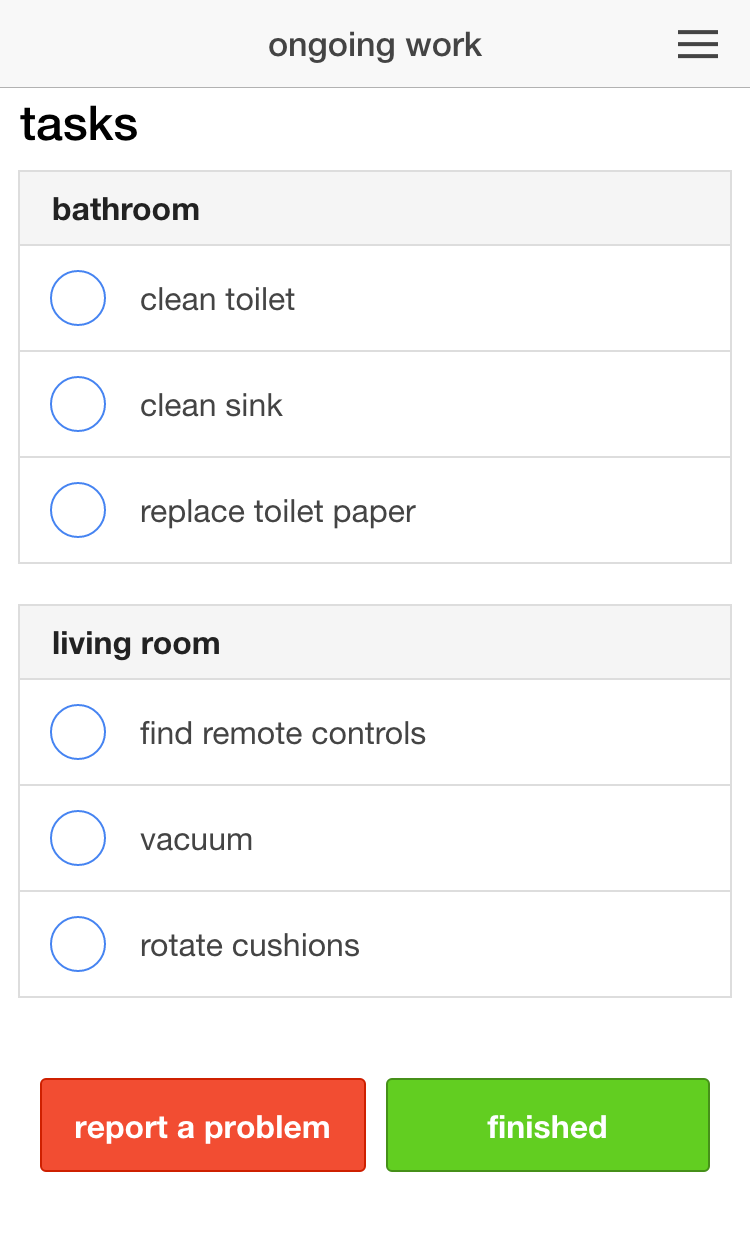
\includegraphics[width=1\columnwidth]{figures/checklist}
    \caption{Explicit checklists make it easier for workers to verify that they've completed all expected work;
    it also makes it apparent to customers that they need to add or clarify certain tasks.}~\label{fig:checklist}
\end{figure}

We tend to agree with this approach.
In our fieldwork we found that paper checklists made it clearer to customers what to expect to be done
--- and importantly, what to expect not to be done.
If customers wanted additional work completed, they could specify that and agree to the extra time it would take to do that job, which they sometimes did.

This ``contract'' between workers and customers can be written collaboratively by both parties,
outlined by the workers themselves, or directed principally by customers as they describe the work they need completed;
the exact process is less important than the shared understanding of the constituent tasks.